\chapter{\Huge{LF7}}\label{ch:lf7}
\section{Grundlagen CPS - Umschalten}\label{sec:lf7_first_Section}
\subsection{Das "Internet der Dinge (engl. "Internet of Things" oder "oT")}\label{subsec:iot)}
\paragraph{Ganz allgemein bezeichnet das Internet der Dinge Alltagsgegenstände, die sowohl mit Ihnen als auch mit anderen Geräten über das Internet kommunizieren.}
\begin{center}
    \begin{figure}[H]
        \centering
        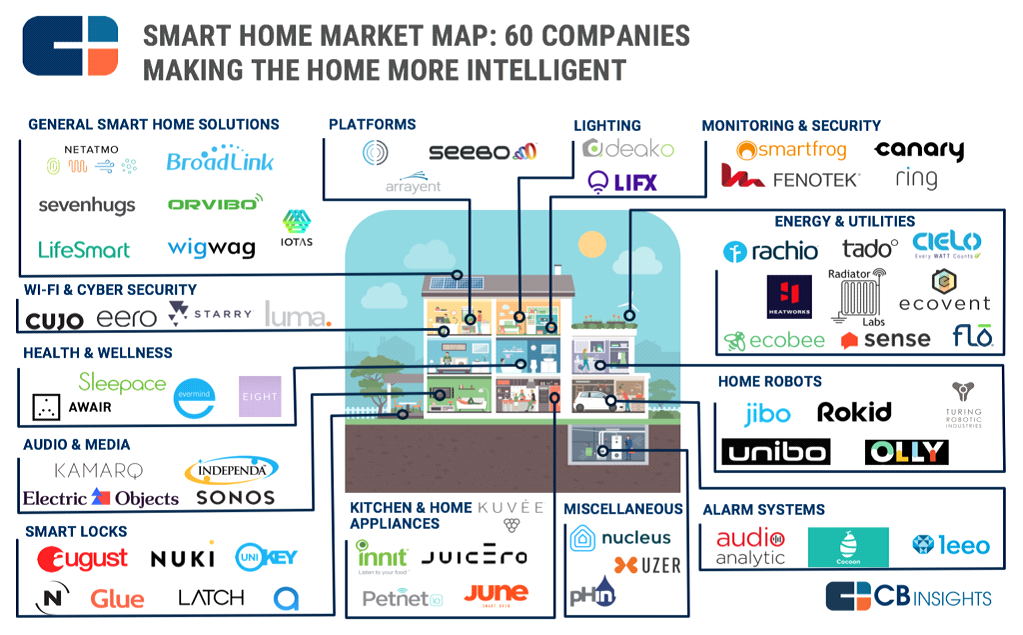
\includegraphics[height=5cm]{imgs/subjects_media/lf7/iot_startups}
        \caption{Smart Home Market Map}\label{fig:figure}
    \end{figure}
\end{center}

\paragraph{Was ist die Vor und Nachteile der Nutzung von Smarthome}

\begin{center}
    \resizebox{\textwidth}{!}{%
        \begin{tabular}{l|l|}
            \hline
            \multicolumn{1}{|l|}{\colorbox{lime}{Vorteile}}                              & \colorbox{orange}{Nachteile}                                                                              \\ \hline
            \multicolumn{1}{|l|}{\colorbox{lime}{Mehr Komfort – mehr Lebensqualität}} &
            \colorbox{orange}{Überwachung} durch IoT Geräte – Vertrauen zum Hersteller \\ \hline
            \multicolumn{1}{|l|}{Überblick wenn man nicht zu Hause ist}          & angreifbar für Bots (wenn öffentlich Verfügbar)                                                 \\ \hline
            \multicolumn{1}{|l|}{\colorbox{lime}{Sparen durch höhere Effizienz} (z.B. Heizung aber Grundverbrauch der Geräte)} &
            \colorbox{orange}{Teuer in der Anschaffung} \\ \hline
            \multicolumn{1}{|l|}{Erhöhte Sicherheit – Überwachung aus der Ferne} & Wartungsintensiv                                                                                \\ \hline
            \multicolumn{1}{|l|}{Barrierefreiheit}                               & Kompatibilitätsprobleme der Hardware                                                            \\ \hline
            \multicolumn{1}{|l|}{Offene Schnittstellen (falls vorhanden)}        & Verfügbarkeit im Internet kann gefährlich sein                                                  \\ \hline
            \multicolumn{1}{|l|}{Gesundheitsvorteile (Luftqualität überwachen)} &
            \colorbox{orange}{Datenschutz} ist ein Problem (z.B. Alexa hört immer zu) \\ \hline
            \multicolumn{1}{|l|}{Personalisierte Automation}                     & komplizierte Bedienung                                                                          \\ \hline
            \multicolumn{1}{|l|}{Bessere WLAN Abdeckung}                         & meist nicht reparabel                                                                           \\ \hline
            & Grenzen bei der Größe der Systeme                                                               \\ \cline{2-2}
            & Probleme bei Funkverbindungen (Zu viele Geräte, schlechte Verbindung, gesundheitlich schädlich) \\ \cline{2-2}
            & nicht in jedem Haus implementierbar                                                             \\ \cline{2-2}
            & \textbf{Sicherheitsbedenken (IoT als Ziel)}                                                     \\ \cline{2-2}
        \end{tabular}%
    }
\end{center}
\paragraph{Viel Komfort -> wenig Sicherheit \\Viel Sicherheit -> wenig Komfort}
\setcounter{section}{0}
\setcounter{figure}{0}